
During experiments, it was found that MVVR (FVR applied to monocular camera sensor data) had considerably less accuracy and robustness than the other FVR methods (FVR, FFVR and FVR-3D). Additionally, we found that MVVR was less robust to rotational transforms. This is due to the fact that depth maps produced by monocular sensor methods, such as optical flow, do not produce sufficiently accurate and reliable depth maps. Results from stereo and active camera tests suggest that this is due to the reduction in accurate and precise depth data generation. \\

Nevertheless, to evaluate the performance of the MVVR method, quantitative experiments were performed on the Kitti Vision Benchmark Data Set. In these experiments, the MVVR method was compared with methods from the literature including FM2D, FM3D. ICP and PCA. Each depth map was projected into volume sizes of $256^3$ for processing by the rest of the MVVR method (the FVR part). To generate the depth maps, a local 2D block matching method was used. Kernel sizes used in the correlation procedure were $3 \times 3$ in size with a search area size of $21 \times 21$. The sizes of the kernel, search area and volume sizes were all chosen empirically. \\

Depth maps computed using the block matching method are only estimates of true scene depth. Therefore, resulting projections are not accurate. These projections, however, are still good enough to produce reconstructions. Registration of these inaccurate projections is difficult due to the amount of noise in the data. Figure \ref{fig:lidarVSMono} shows the noise contrast between depth maps produced by a LIDAR and a monocular block-matching system. \\

\begin{figure}[!htb]
\centering
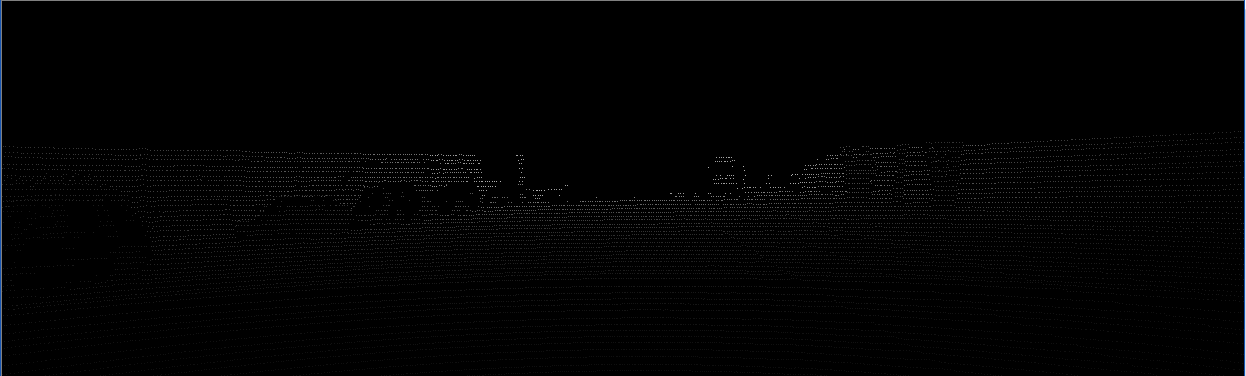
\includegraphics[width=4.5in]{images/methodology/FVR/mono/color}

\includegraphics[width=4.5in]{images/methodology/FVR/mono/depth}
\caption{Top: Ground Truth Depth Map Computed Using a LIDAR System, Bottom: Depth Map Computed Using a Monocular Method (inverted)}
\label{fig:lidarVSMono}
\end{figure}


Results on the Kitti Benchmark 0001 Sync data set are shown in Table \ref{table:MVVRQuantitativeExperimentResults}. In these results, ICP outperformed the other methods, with each algorithm having larger errors due to the inaccurate depth maps. Here, FVR achieved the best result ~29.25 \% of the time. Compared to results in Table \ref{tab:kittidata0001sync}, the MVVR method was less competitive than ICP. Due to the low-quality projections, FM2D and PCA failed were not able to register every frame. Most of the algorithms had incorrectly registered frames at some point.

\begin{table}[t]
\centering
\caption{Reconstruction Errors for the Kitti Data 0001 Sync Data Set Using Monocular (RGB) Input Only}
\begin{tabular}{ccc}
\hline
\textbf{Algorithm} & \textbf{Median Error $\times$ 1000} & \textbf{\% best results}\\ \hline
FM2D	& 3742.4 & 2.83\%\\
FM3D	& 918.05 & 14.15\%\\
ICP	& 772.48 & 50.94\%\\
PCA	& 2046.96 & 2.83\%\\
MVVR	& 944.81 & 29.25\%\\
\end{tabular}
\label{table:MVVRQuantitativeExperimentResults}
\end{table} 

These results, and those from the Stereo and Active camera experiments, indicate that, if the quality of the depth maps had been higher, the FVR based methods would have produced better results. \\
